% Latex template: mahmoud.s.fahmy@students.kasralainy.edu.eg
% For more details: https://www.sharelatex.com/learn/Beamer

\documentclass[1611]{beamer}					  % Document class

\usepackage[portuguese]{babel}			  % Set language
\usepackage[utf8x]{inputenc}			  % Set encoding

\mode<presentation> {					  % Set options
  \usetheme{default}					    % Set theme
  \usecolortheme{default} 				% Set colors
  \usefonttheme{default}  				% Set font theme
  \setbeamertemplate{caption}[numbered]	% Set caption to be numbered
}

\setbeamertemplate{navigation symbols}{}
\setbeamertemplate{footline}[frame number]
\setbeamercovered{transparent}

\newcommand\Wider[2][3em]{%
\makebox[\linewidth][c]{%
  \begin{minipage}{\dimexpr\textwidth+#1\relax}
  \raggedright#2
  \end{minipage}%
  }%
}

% Uncomment this to have the outline at the beginning of each section highlighted.
%\AtBeginSection[]
%{
%  \begin{frame}{Outline}
%    \tableofcontents[currentsection]
%  \end{frame}
%}

\usepackage{graphicx}					% For including figures
\usepackage{booktabs}					% For table rules
\usepackage{hyperref}					% For cross-referencing
\usepackage{caption}                    % Allows more control over captions in figs and tables

\title{Revisão de Atividades da FAC}	% Presentation title
%\author{Author One}					% Presentation author
\institute{LNLS.DAC.FAC}				% Author affiliation
\date{2024-03-08 -- 2024-04-19}			% Today's date	


\begin{document}



\begin{frame}
  \titlepage
  \href{https://github.com/lnls-fac/doc-review-dac-fac}{\beamergotobutton{Link para o repo github desta apresentação: https://github.com/lnls-fac/doc-review-dac-fac}}
  \href{https://www.overleaf.com/read/sbdjxtzfchrm}{\beamergotobutton{Link para o projeto overleaf destas notas}}
\end{frame}

\begin{frame}{Outline}
  \tableofcontents
\end{frame}

% Machine studies in the period

% 2024-03-11-FOFB-Acq
% 2024-03-12-SI_llrf_study
% 2024-03-19-SI_NLK
% 2024-03-19-SI_bpms_equalization
% 2024-03-22-SI_hla_problem
% 2024-03-25-SI_FOFB_Study
% 2024-03-25-SI_FOFB_respmat_alternatives
% 2024-03-25-SI_llrf_study
% 2024-03-25-SI_tune-tracking-sigmay-control
% 2024-04-01-BO_beam_images_at_screens
% 2024-04-01-SI_injection_collimation_with_scrapers
% 2024-04-01-SI_orbit_stability_hydraulic_valve_10hz_problem
% 2024-04-12-coldbox-orbit-acqs
% 2024-04-16-SI-delta-optics-ffwd
% 2024-04-16-SI_NLK
% 2024-04-16-SI_boramp_effect_orbit_acq

%====================================================================
\section{Estudos com LLRF}

\begin{frame}
    \Huge{Estudos com LLRF}
\end{frame}

\begin{frame}{Estudos de máquina}
\begin{itemize}
    \item 2024-03-12 $\to$ explorar parâmetros de controle, medidas para paper IPAC, crosstalk entre FOFB e LLRF observado
    \item 2024-03-25 $\to$ explorar crosstalk entre FOFB e LLRF

    \item Parâmetros de operação atuais: \\
    Ki = 8000, Kp = 155, Ph. Shifter: 111°
\end{itemize}
\end{frame}

\begin{frame}{}
\centering
\Wider[4em]{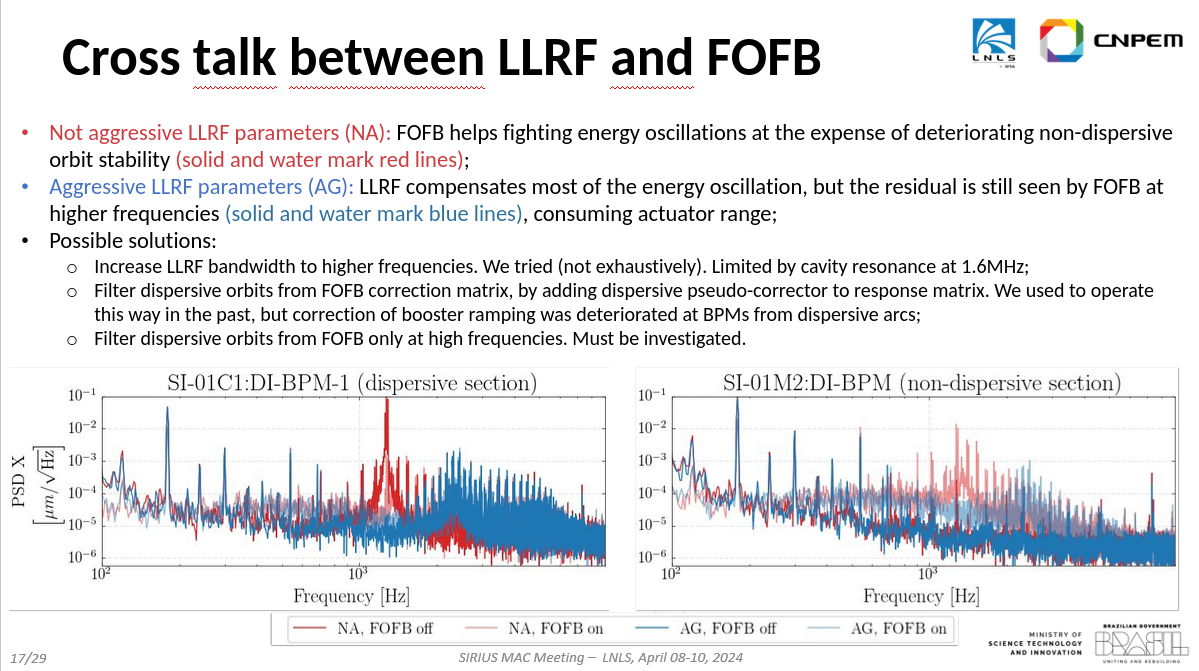
\includegraphics[scale=0.29]{2024-04-19/figures/crosstalk_llrf_fofb.png}}
\end{frame}

%====================================================================
\section{Testes de controle de emitância com bunch-by-bunch}

\begin{frame}
    \Huge{Testes de controle de emitância com bunch-by-bunch}
\end{frame}

\begin{frame}{}
\small{Tune tracking com BbB. Drive feixe em sideband sincrotron à frequência bétatron vertical. Tamanho vertical ajustado de acordo com amplitude do drive. Tempo de vida também variou, significa que de fato o tamanho variou, não é apenas oscilação do centroide.}
\centering
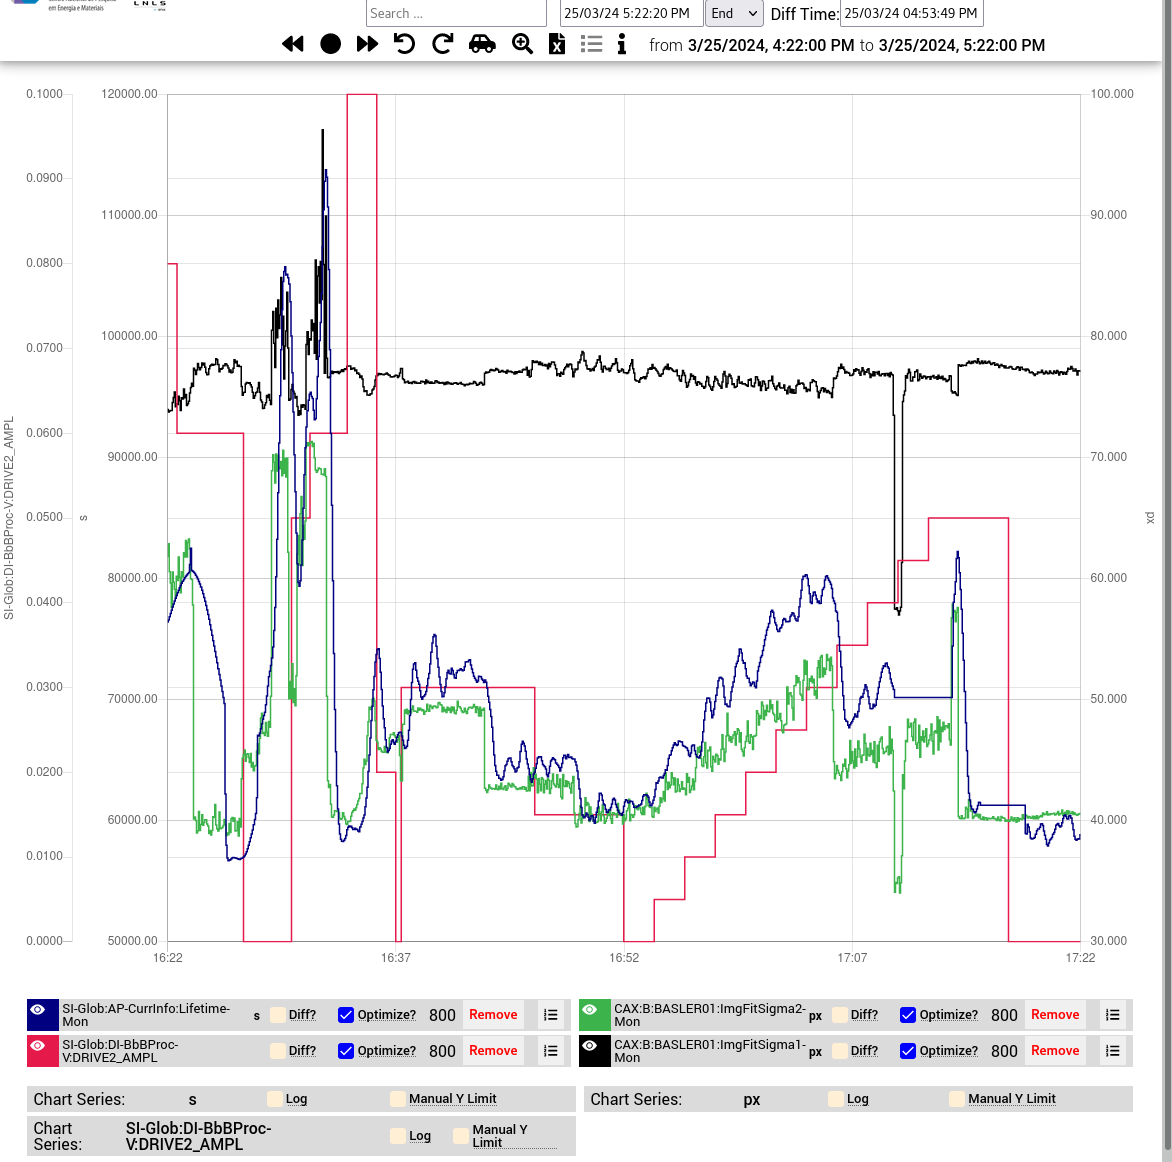
\includegraphics[width=0.7\textwidth]{2024-04-19/figures/emittance_control.png}
\end{frame}


%====================================================================
\section{Testes de colimação com scrapers}

\begin{frame}
    \Huge{Testes de colimação com scrapers}
\end{frame}

\begin{frame}{Scraper vertical}
    \centering
    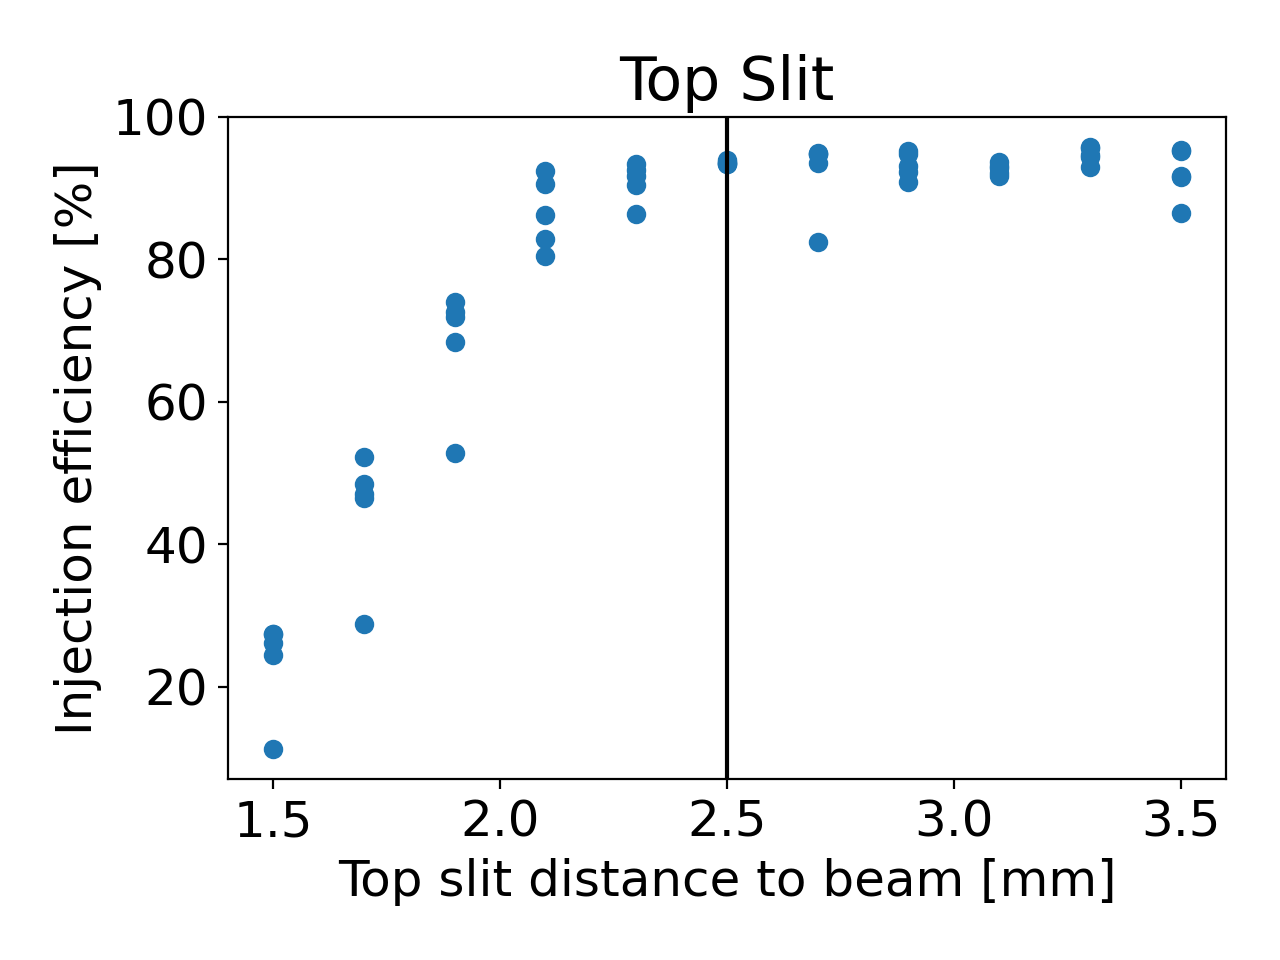
\includegraphics[width=0.5\textwidth]{2024-04-19/figures/Top.png}
    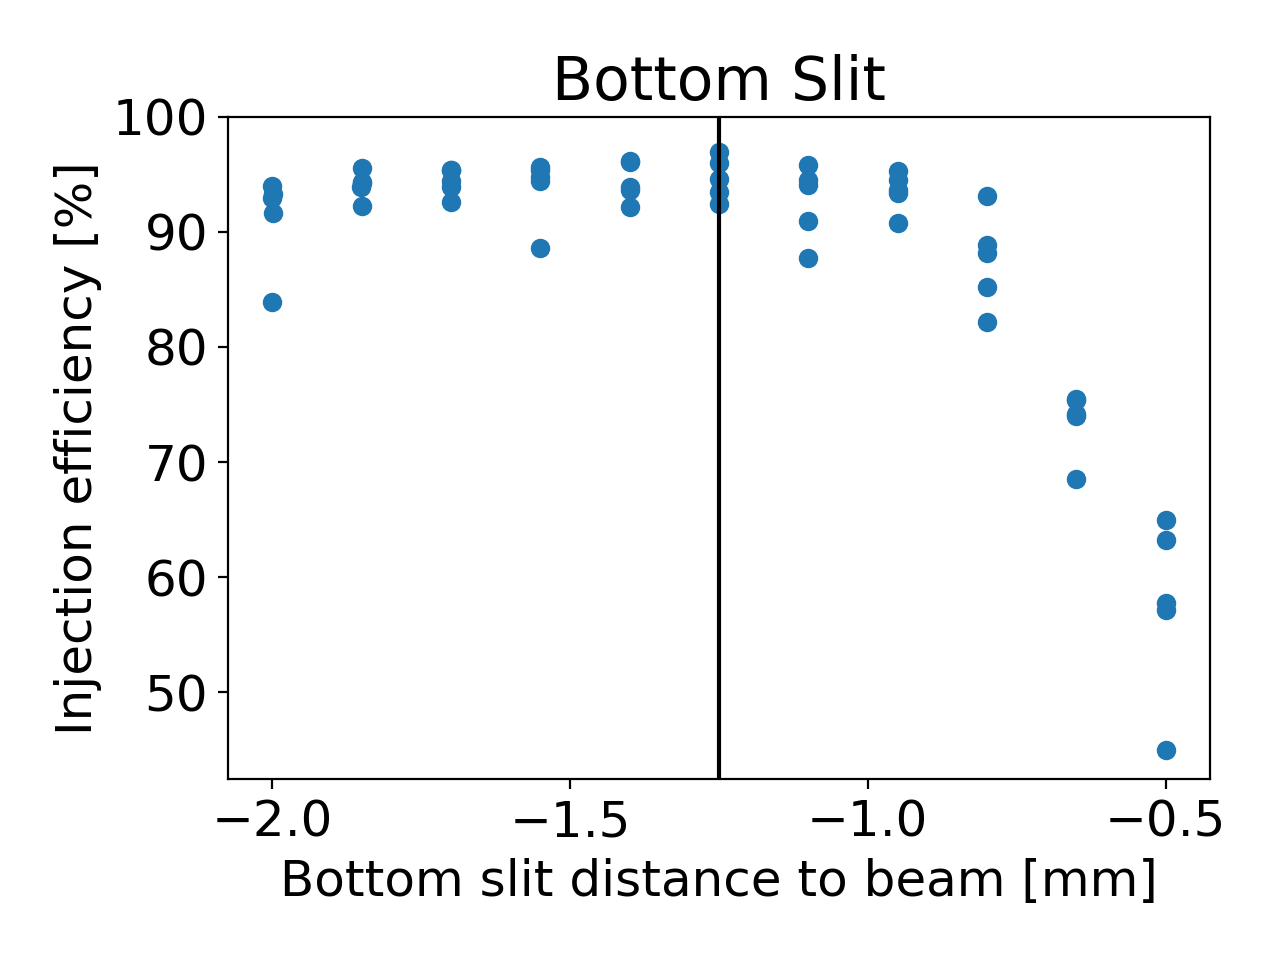
\includegraphics[width=0.5\textwidth]{2024-04-19/figures/Bottom.png}
    \\
    \centering
     Adjusted $\to$ Top: 2.5mm, Bottom: -1.25mm
\end{frame}

\begin{frame}{Scraper horizontal}
    \centering
    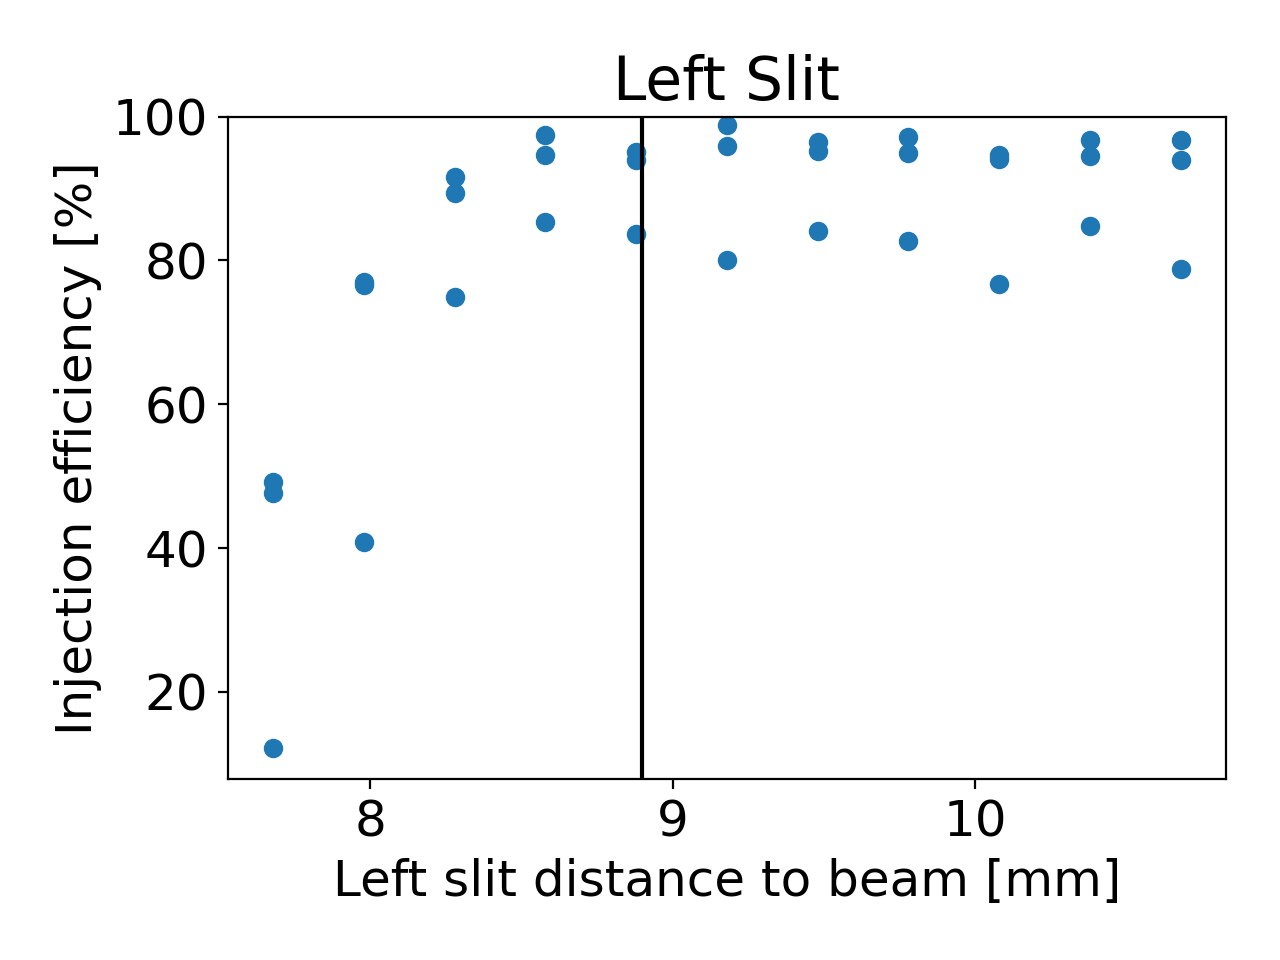
\includegraphics[width=0.48\textwidth]{2024-04-19/figures/Left.png}
    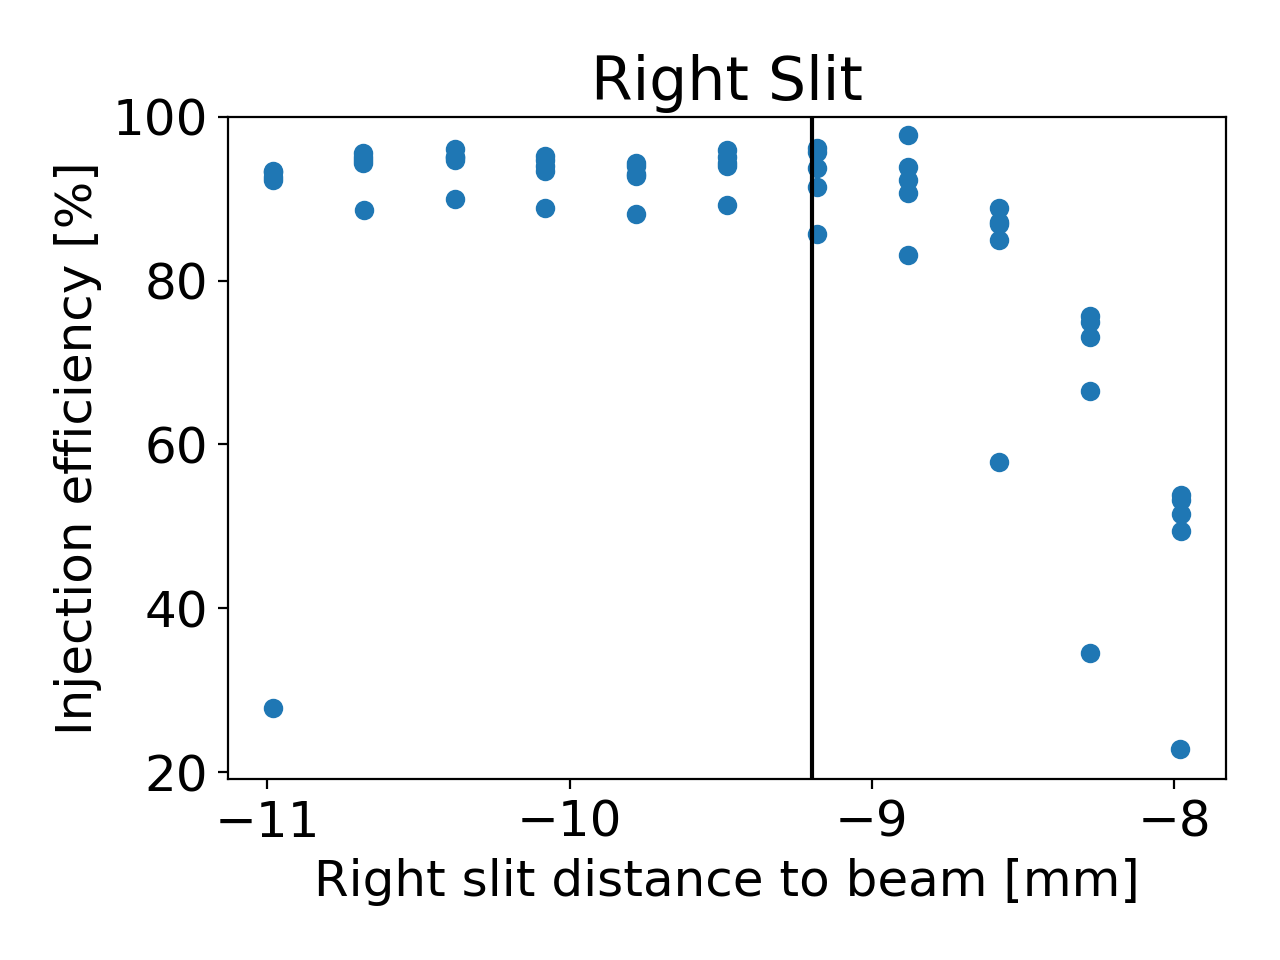
\includegraphics[width=0.48\textwidth]{2024-04-19/figures/Right.png}

     Adjusted $\to$ Left: 8.9mm, Right: -9.2mm
\end{frame}

\begin{frame}{Proteção contra erros de injeção}
Scrapers posicionados em: top 2.5mm, -1.25mm bottom, 8.9mm left, -9.2mm right
\begin{itemize}
    \item  Erros $\theta_x <0$: até -0.5 mrad protege
    \item Erros $\theta_x>0$: até 0.3mrad ou para scrapers abertos, perdas se concentram em torno dos trechos 12 ou 13
    \item Erros $\theta_y<0$: não protege range -(0.3, 0.4) mrad
    \item Erros $\theta_y>0$: range de (0.2, 0.4) mrad
    
    
    \item Erros $x < 0$: protege relativamente no range de (0, -1.0) mm
    \item Erros $x >0$: protege no range de (0, 1.0) mm
    
    \item Erros $y > 0$: protege em (0.5, 0.7) mm
\end{itemize}
Subimos a corrente para 100 mA, scrapers nestas posições definidas, sem afetar o tempo de vida.

Para operação voltamos os scrapers para máxima abertura.
\end{frame}

%====================================================================
\section{Estabilidade de órbita}
\begin{frame}
    \Huge{Estabilidade de órbita}
\end{frame}

\begin{frame}{O mistério em 10Hz}
2024-04/01: Medidas para MAC Meeting, novo pico em 10Hz
\centering
    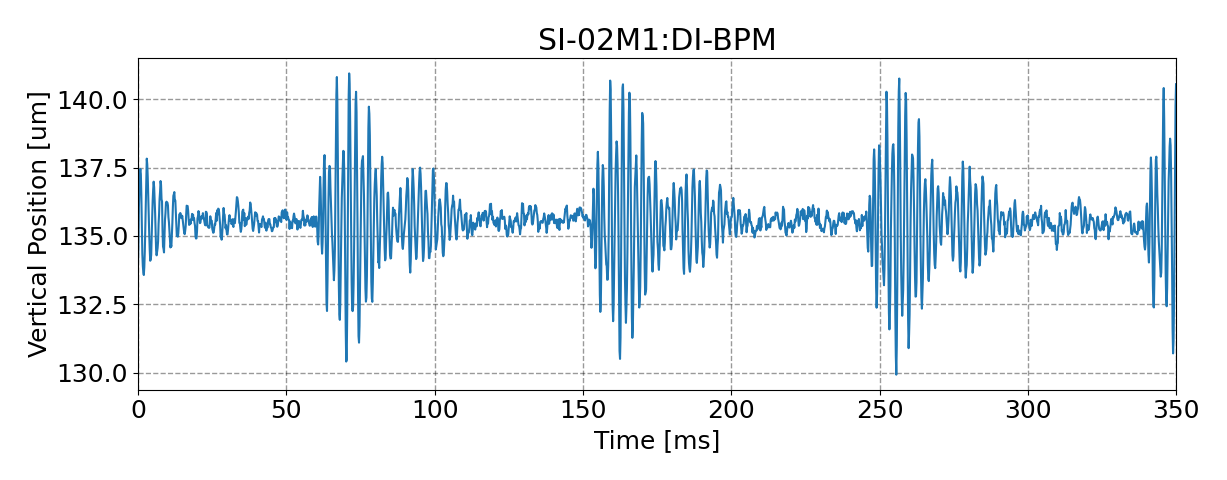
\includegraphics[scale=0.3]{2024-04-19/figures/bpm_data_rate_facq_sofbstate_on_fofbstate_on_gain_0p052_rfline_off_llrf_ki_8000_kp_155_vert_orb_at_01M2.png}
    \\
Sinal convertido para áudio. Similar a um som de compressor
\end{frame}

\begin{frame}{Localização do efeito no trecho 10SB}
\centering
    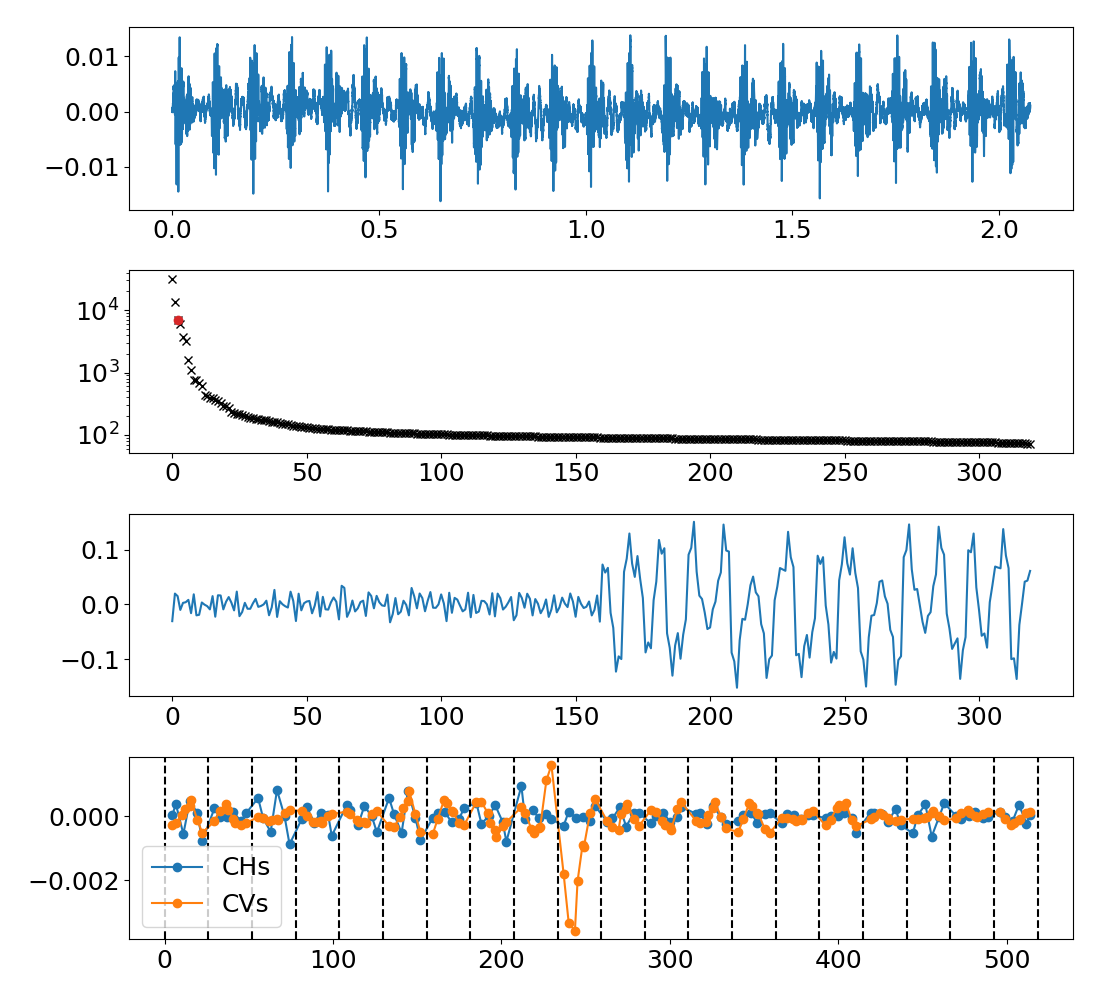
\includegraphics[scale=0.25]{2024-04-19/figures/bpm_data_rate_fofb_sofbstate_off_fofbstate_off_gain_0p052_rfline_off_llrf_ki_8000_kp_155.png}

Entrada no túnel, válvula com problema no trecho 10SB gerando vibração nas mangueiras e em todo berço. Resolvido problema com a válvula.
\end{frame}

%====================================================================
\section{MAC Meeting}

\begin{frame}
    \Huge{MAC Meeting}\\
    \normalsize{08-10 de Abril}
\end{frame}

\begin{frame}{Apresentações FAC}
    \begin{itemize}
        \item 03 - Beam Stability
        \item 08 - Progress on Third Harmonic Cavities Studies
        \item 13 - Injection System
        \item 14 - Nonlinear Dynamics
    \end{itemize}

    Relatório final com comentários e recomendações do MAC está disponível
\end{frame}

%====================================================================
\section{Estudos 2023-04-16}

\begin{frame}{Estudos 2023-04-16}
    \begin{itemize}
        \item Feedforward de ótica do Delta
        \item Ajustes com nova eletrônica NLK (maior range de tensão)
        \item Feedforward com corretoras do anel para compensar perturbação do Booster (múltiplos de 2Hz)
        \item Bunch-cleaning com feedback positivo na vertical
    \end{itemize}
\end{frame}


%====================================================================
\section{Feedforward de óptica do Delta}

\begin{frame}{Medidas de matriz resposta}
  \begin{figure}[ht]
        \begin{minipage}[b]{0.45\linewidth}
            \centering
            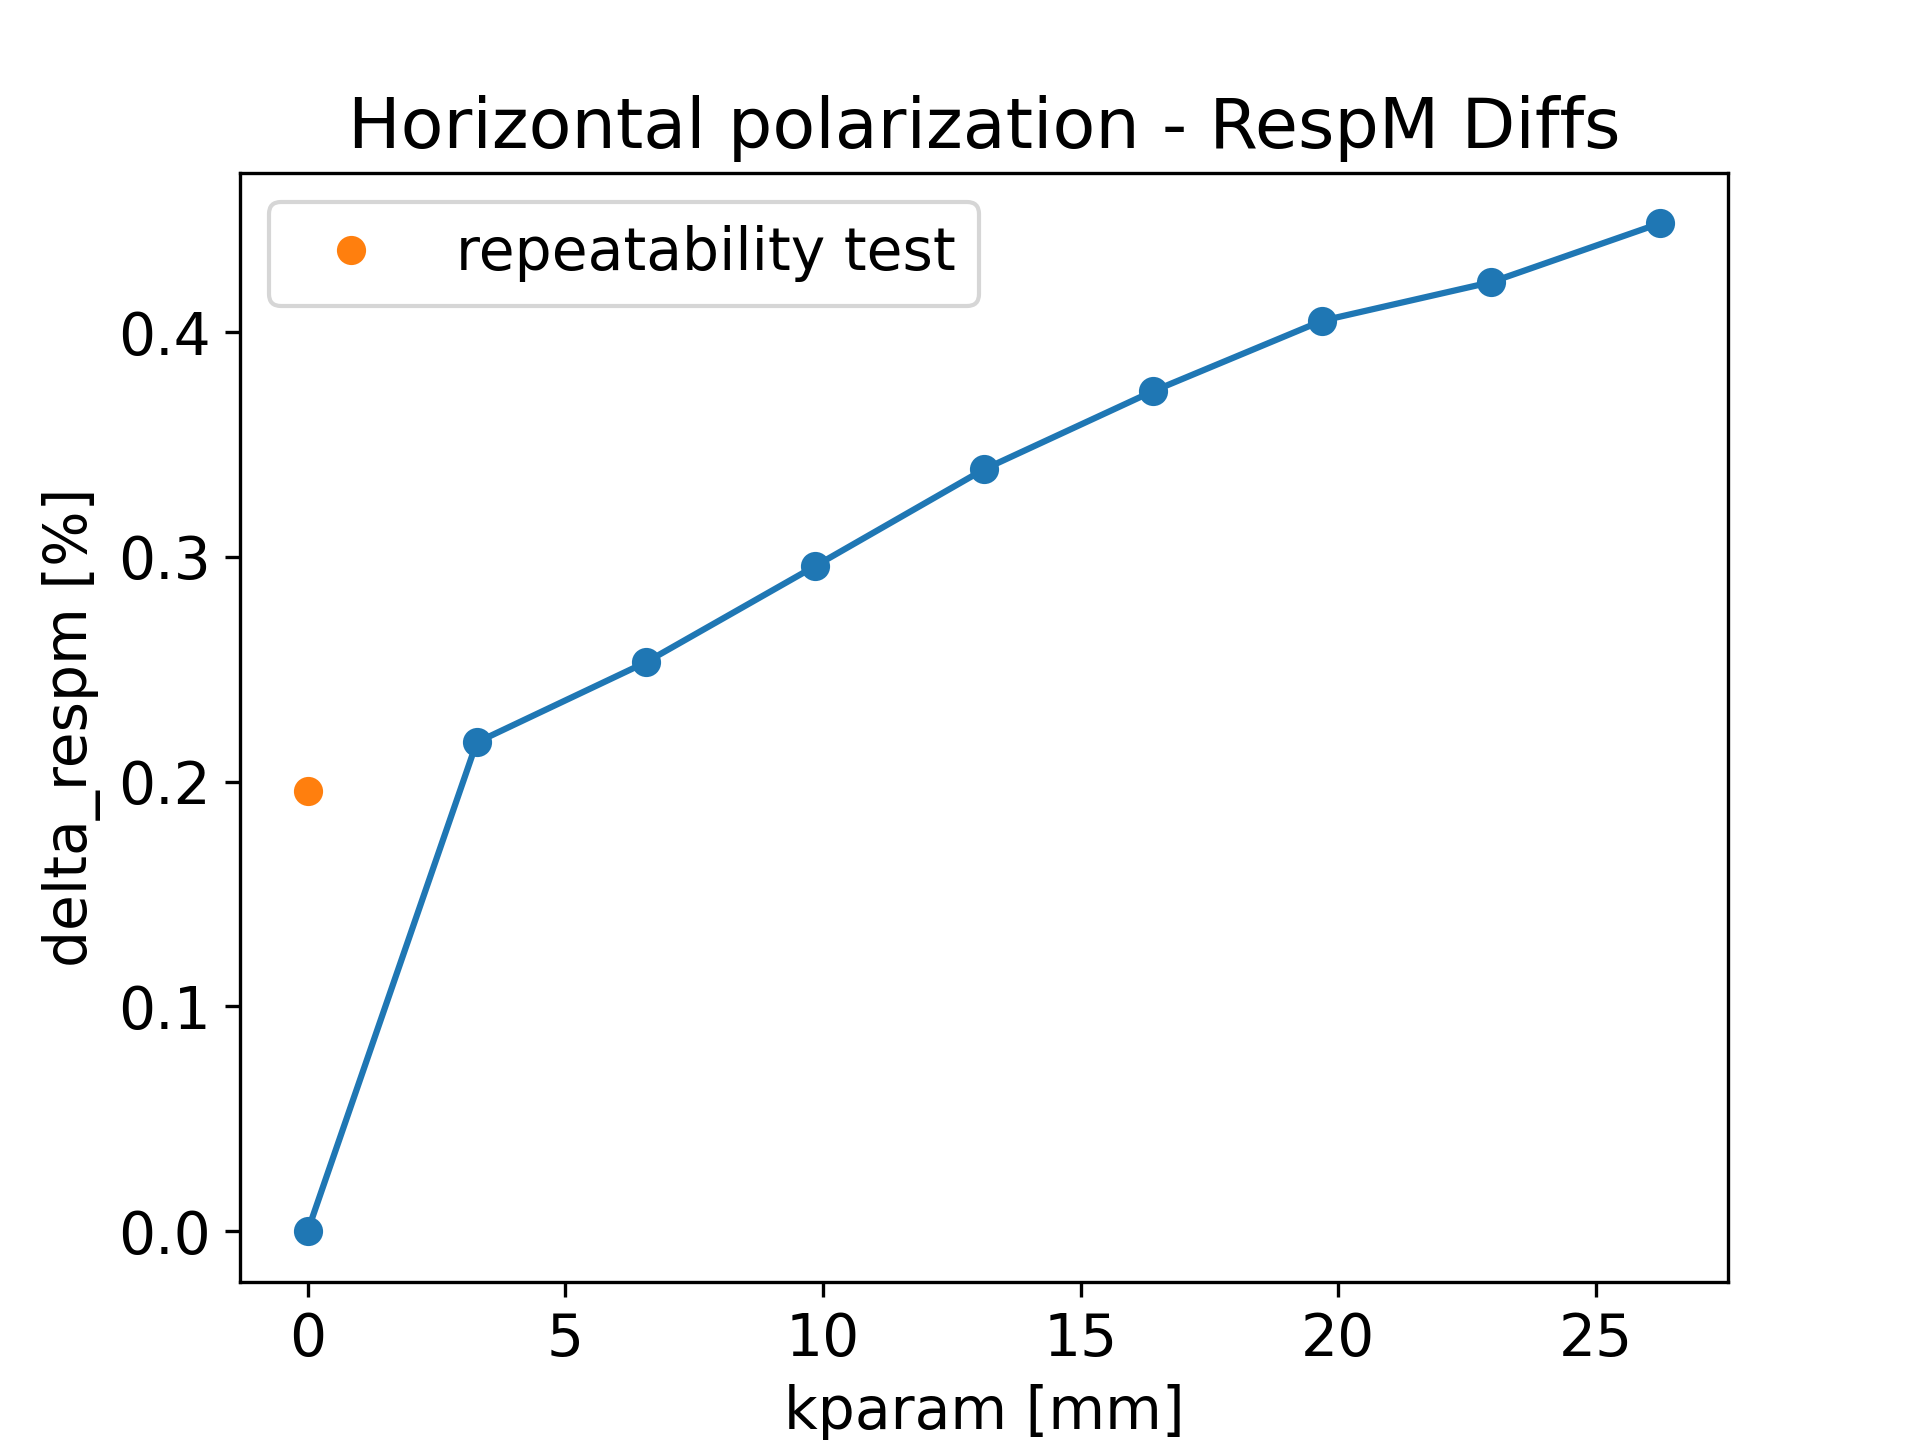
\includegraphics[width=\textwidth]{2024-04-19/figures/repeatability.png}
            \caption{Comparação do efeito do Delta na matriz resposta com repetibilidade da medida.}
            \label{fig:a}
        \end{minipage}
        \hspace{0.5cm}
        \begin{minipage}[b]{0.45\linewidth}
            \centering
            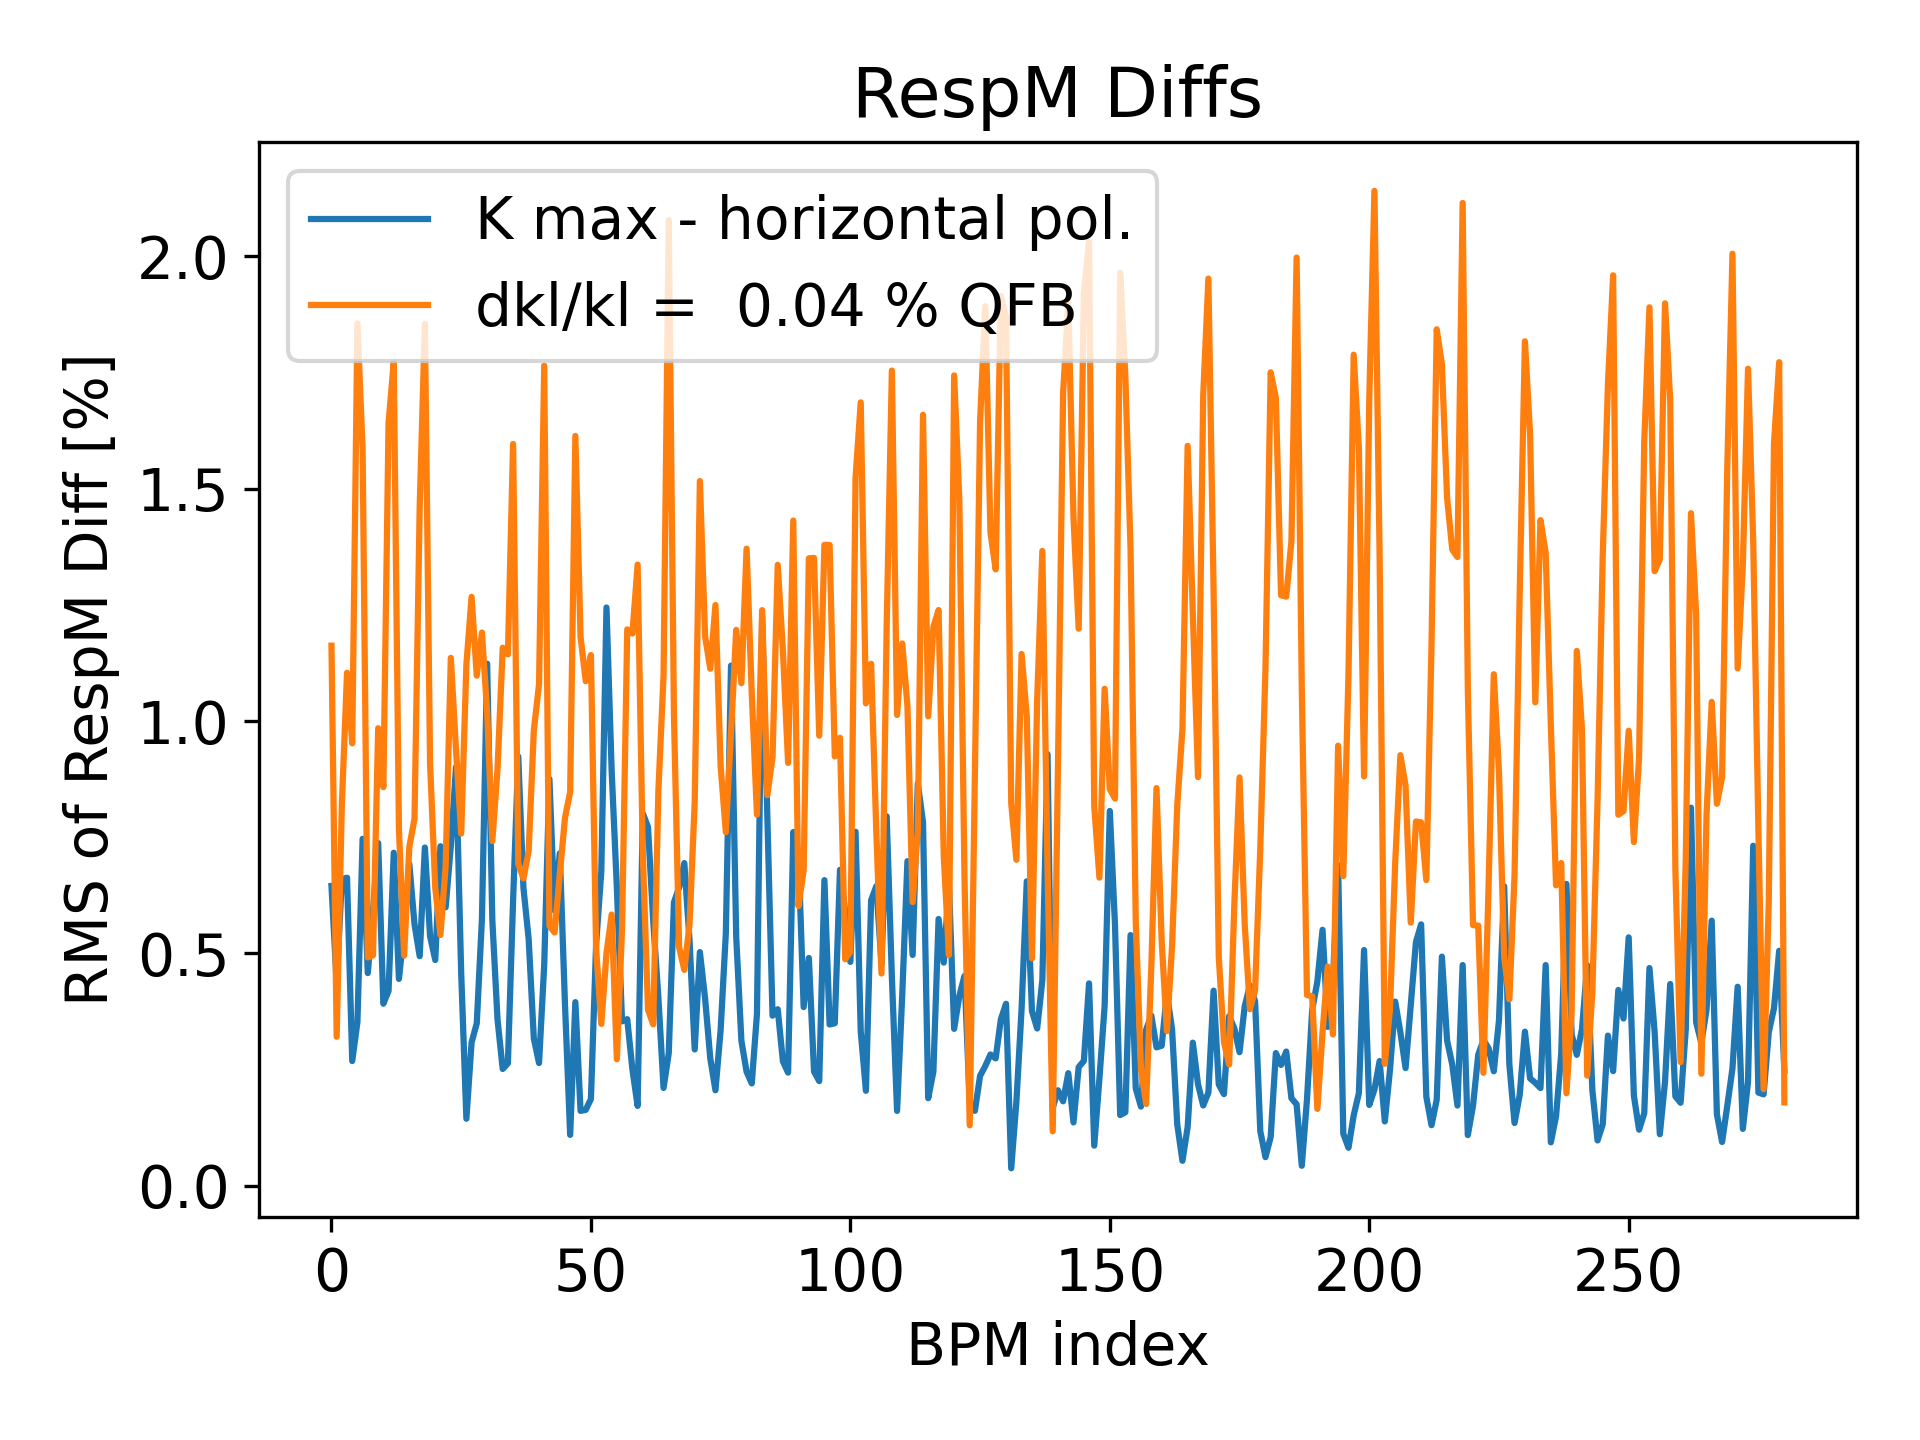
\includegraphics[width=\textwidth]{2024-04-19/figures/Matrix_diff.png}
            \caption{Comparação entre efeito da variação de KL e efeito do Delta na matriz resposta.}
            \label{fig:b}
        \end{minipage}
   \end{figure}
O método de fitting não tem resolução para fitar as variações de KL induzidas. Resolução da medida é da ordem de 0.03 \%.
\end{frame}

\begin{frame}{Correção da variação de sintonia com quadrupolos locais}
    \begin{figure}[ht]
        \begin{minipage}[b]{0.45\linewidth}
            \centering
            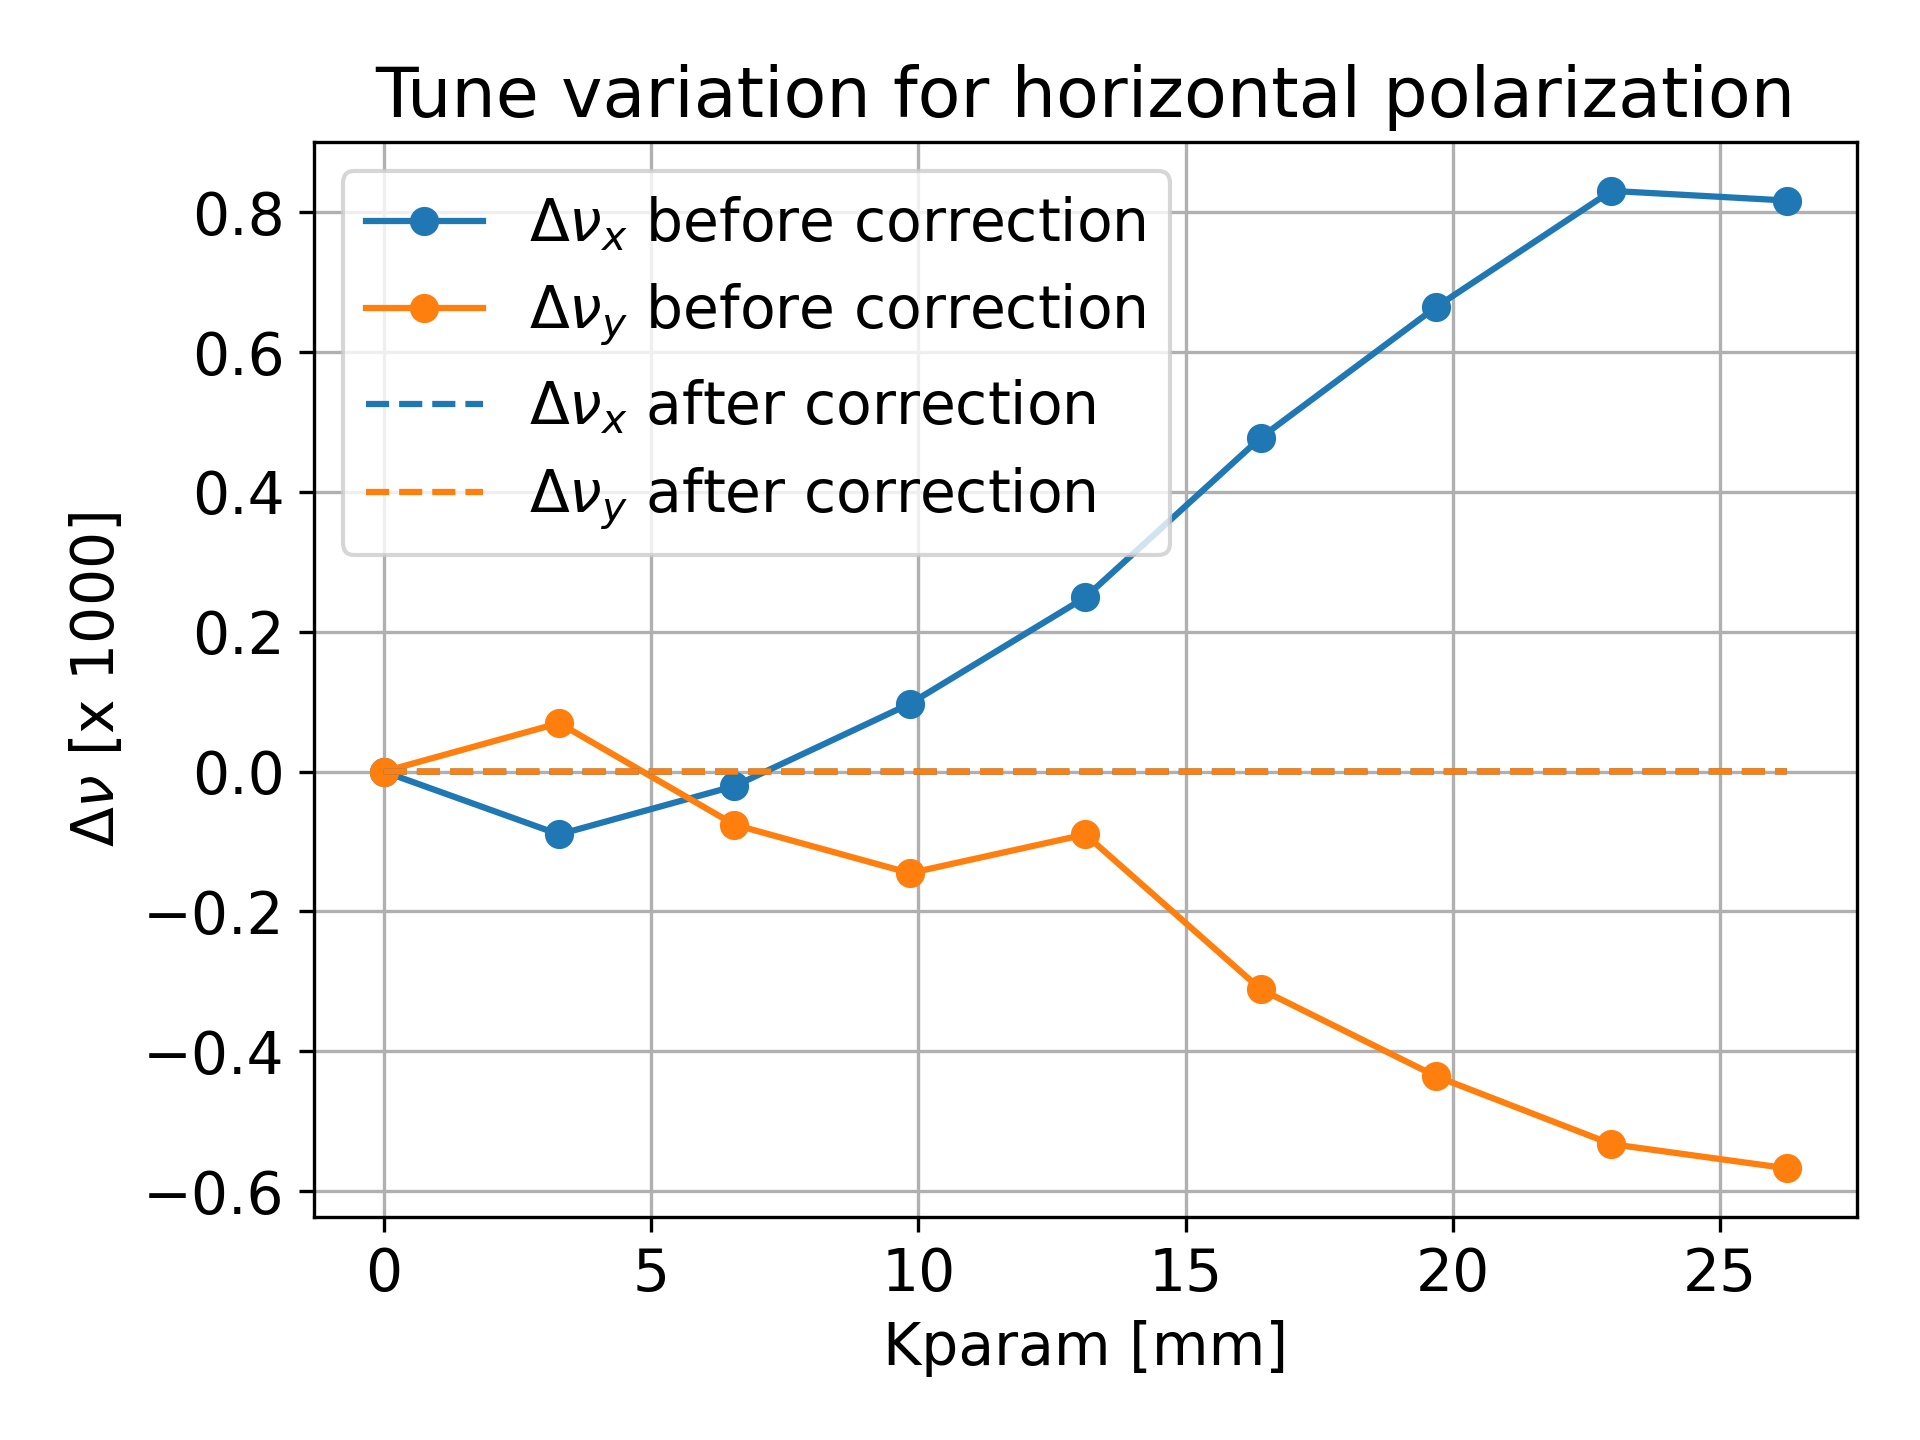
\includegraphics[width=\textwidth]{2024-04-19/figures/tune_corr_model.png}
            \caption{Correção das variações de sintonia usando modelo fitado.}
            \label{fig:a}
        \end{minipage}
        \hspace{0.5cm}
        \begin{minipage}[b]{0.45\linewidth}
            \centering
            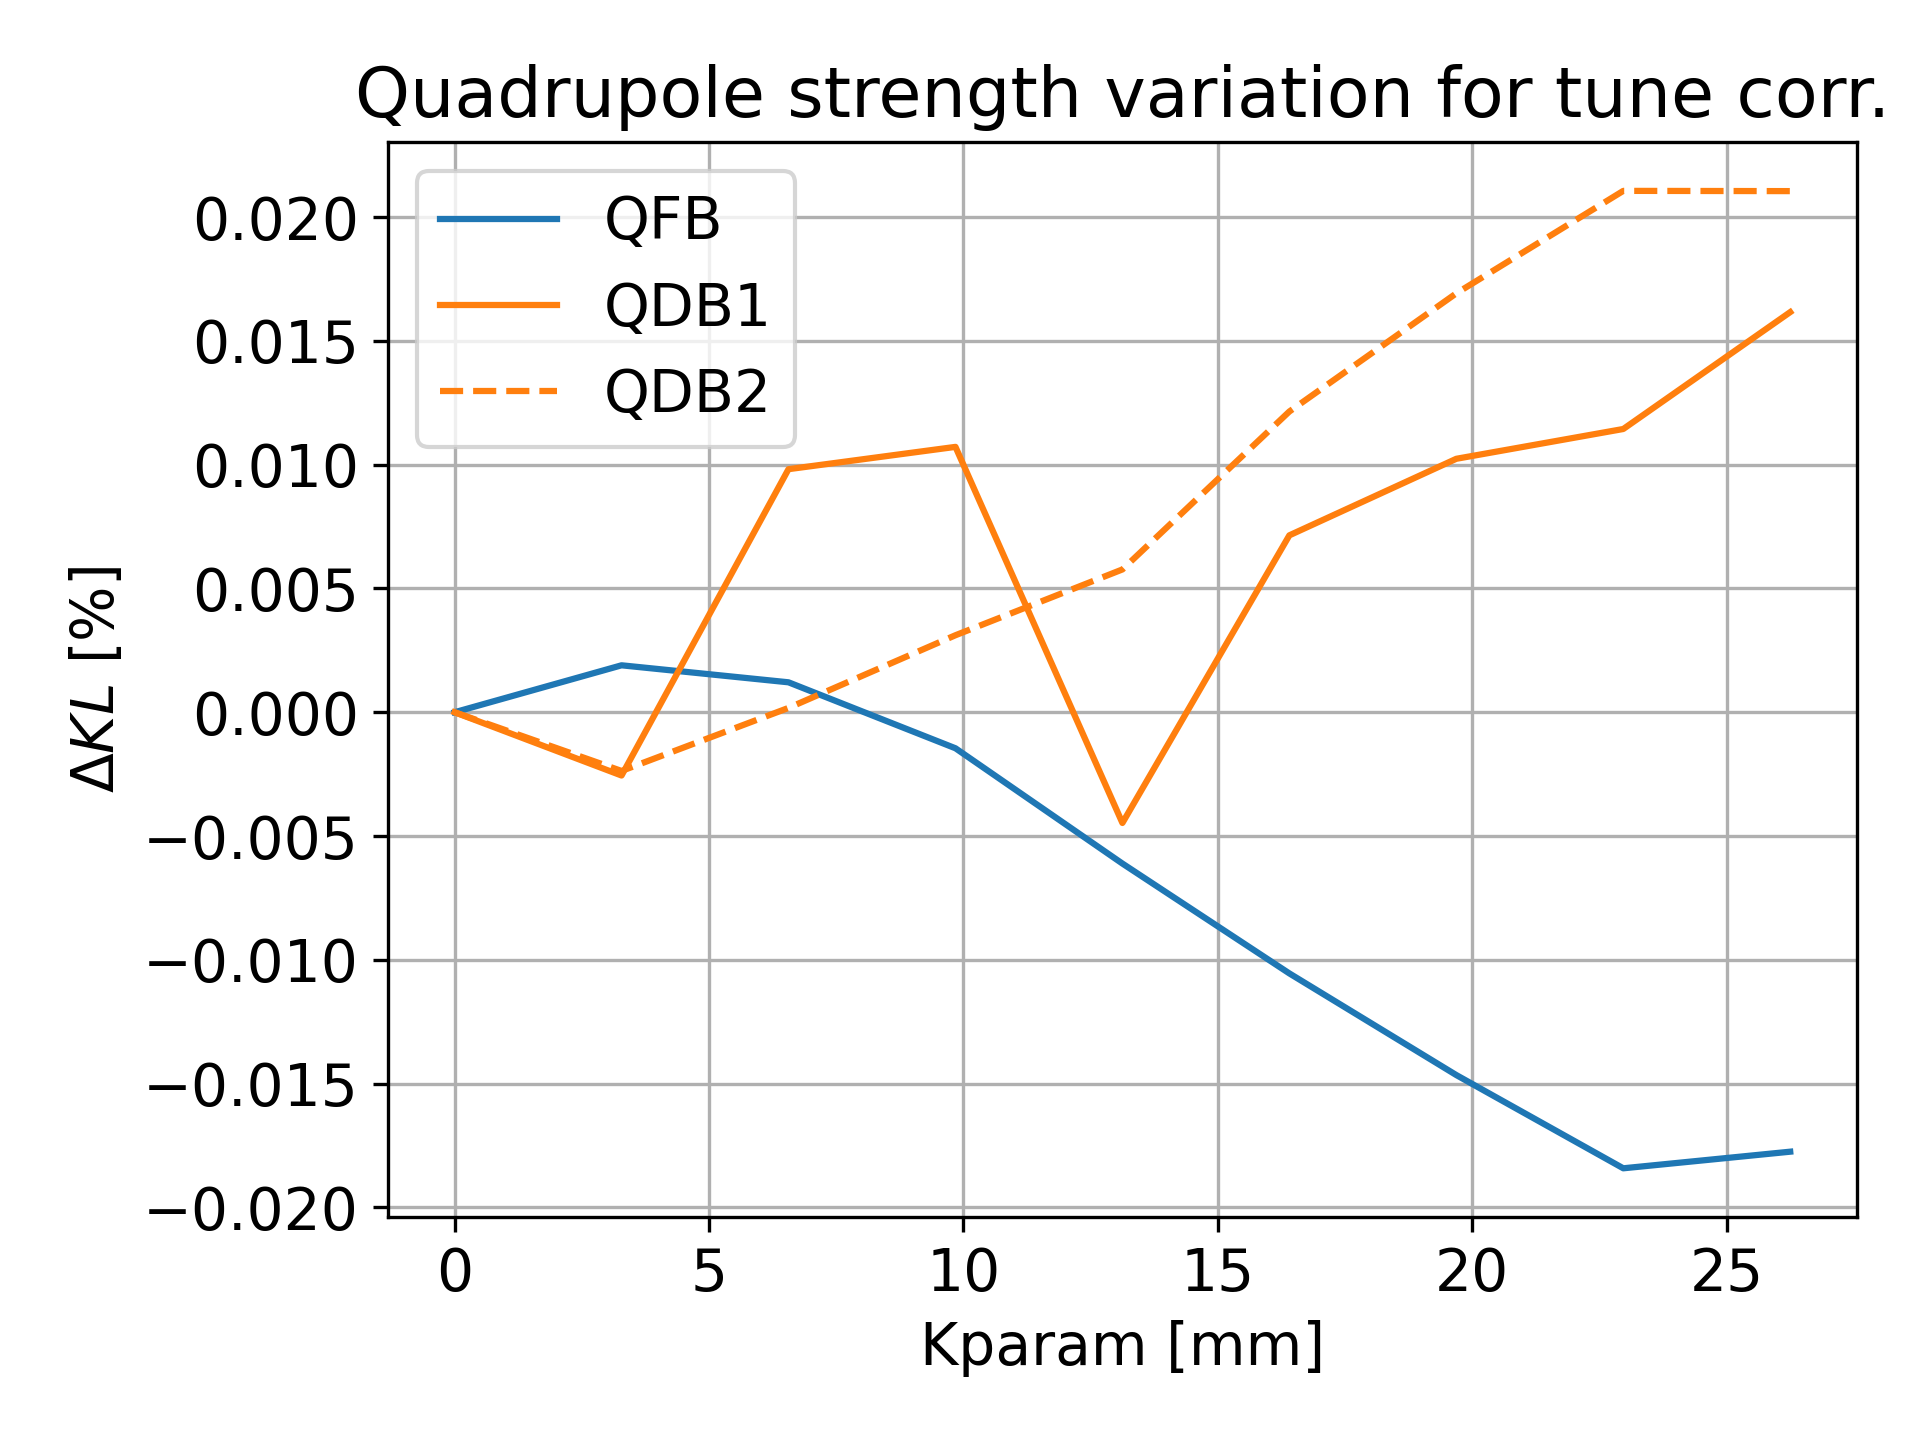
\includegraphics[width=\textwidth]{2024-04-19/figures/Quad_stg.png}
            \caption{Variação forças dos quadrupolos necessárias para correção.}
            \label{fig:b}
        \end{minipage}
    \end{figure}
As variações das forças em geral são menores do que 0.02\%.
\end{frame}

\begin{frame}{Realinhamento NLK}
Variação de 100$\mu$m na horizontal
\centering
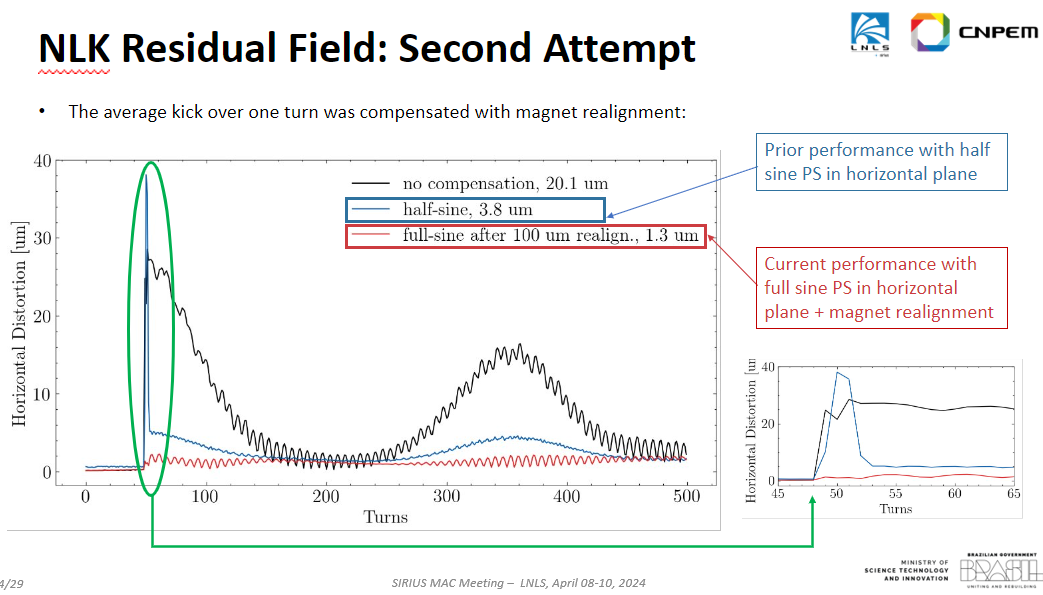
\includegraphics[scale=0.6]{2024-04-19/figures/nlk_perturb.PNG}
    
\end{frame}

\begin{frame}{Compensação NLK}
\begin{itemize}
    \item Bastidor alterado para maior range de tensão. Antigo estava operando no máximo (200V setpoint sala de controle).
    \item Ajuste do amplitude e delay para melhor reproduzir referência no osciloscópio \\
    CoilH: Amp. 97V, DeltaDelay -0.12$\mu$s em relação ao NLK

    \centering
    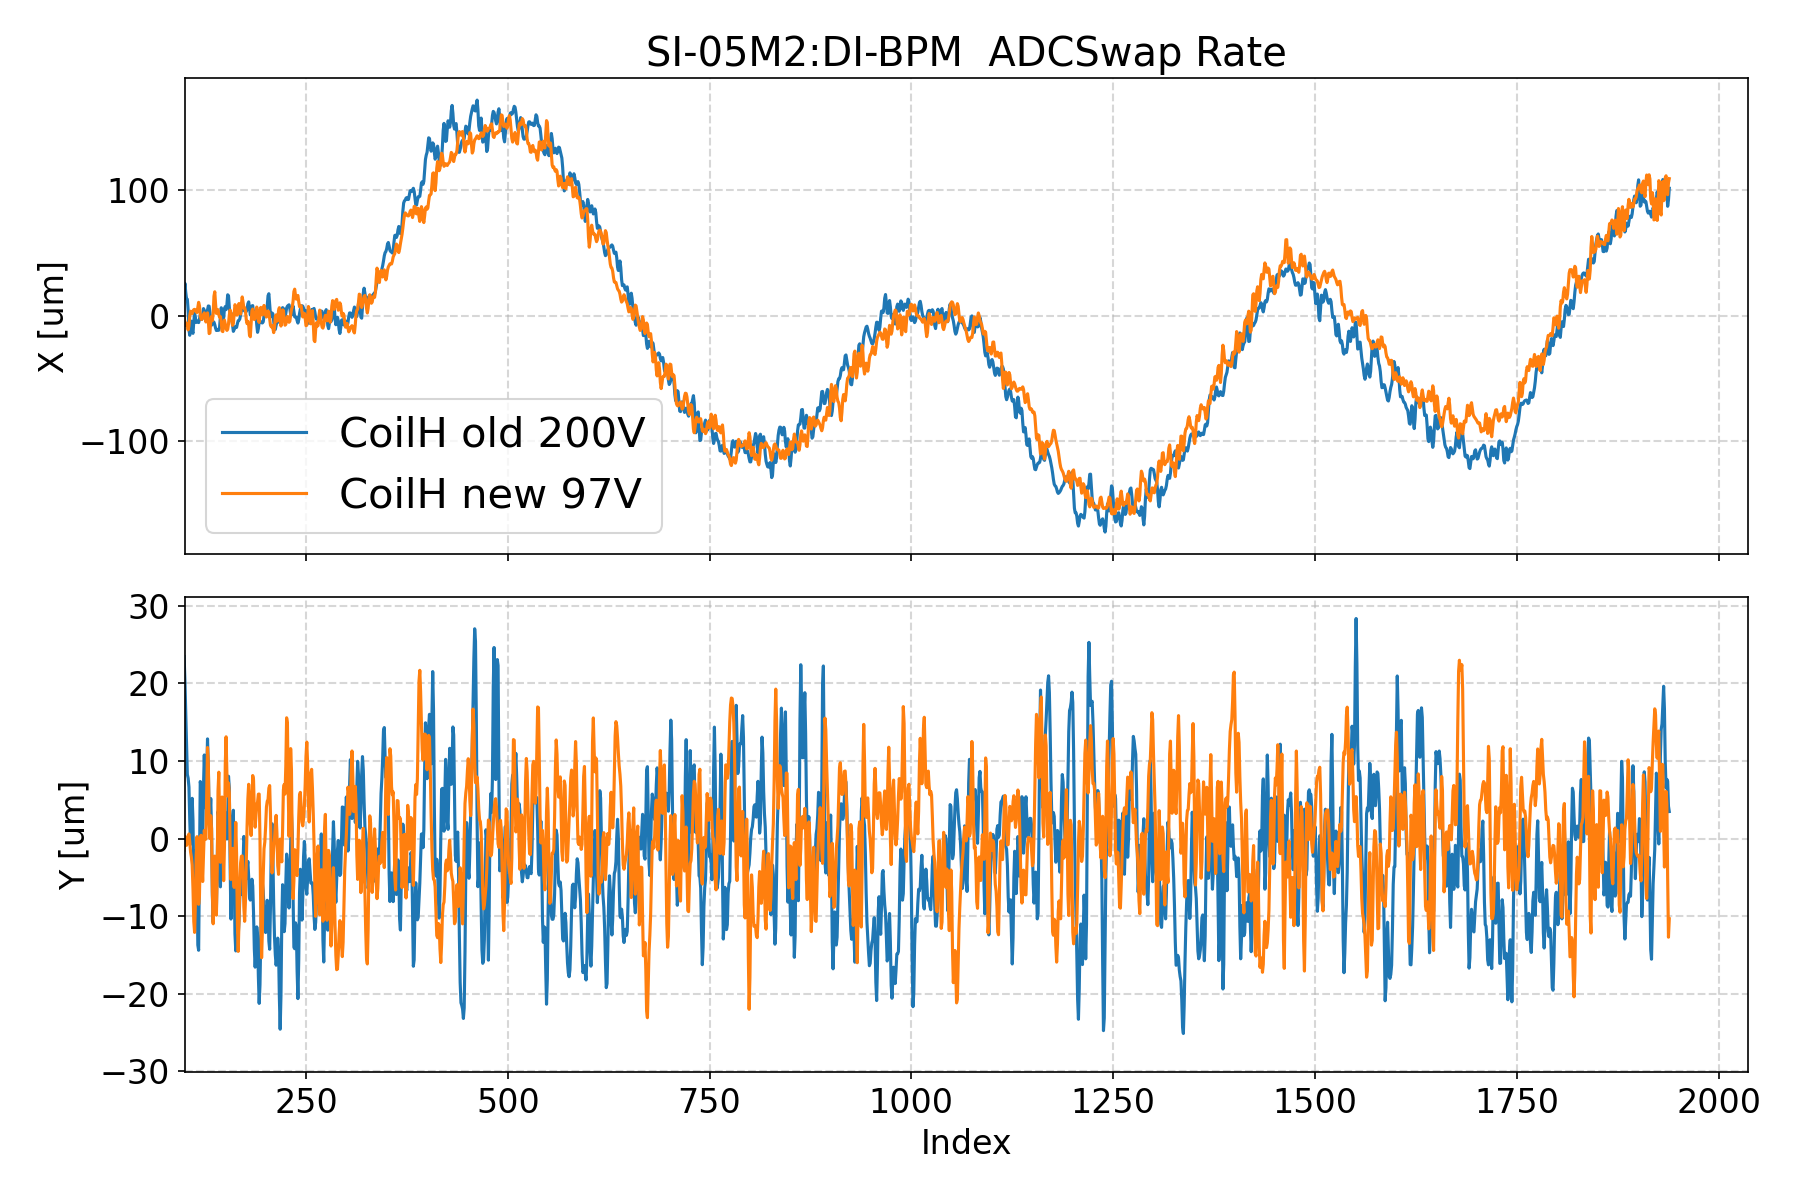
\includegraphics[width=0.8\textwidth]{2024-04-19/figures/coilh_old_new.png}
\end{itemize}
\end{frame}

\begin{frame}{Diferença da compensação}
\centering
    Neste BPM \\
    media 1.6$\mu$m $\to$ 2.6$\mu$m\\
    rms 19$\mu$m $\to$ 24$\mu$m
    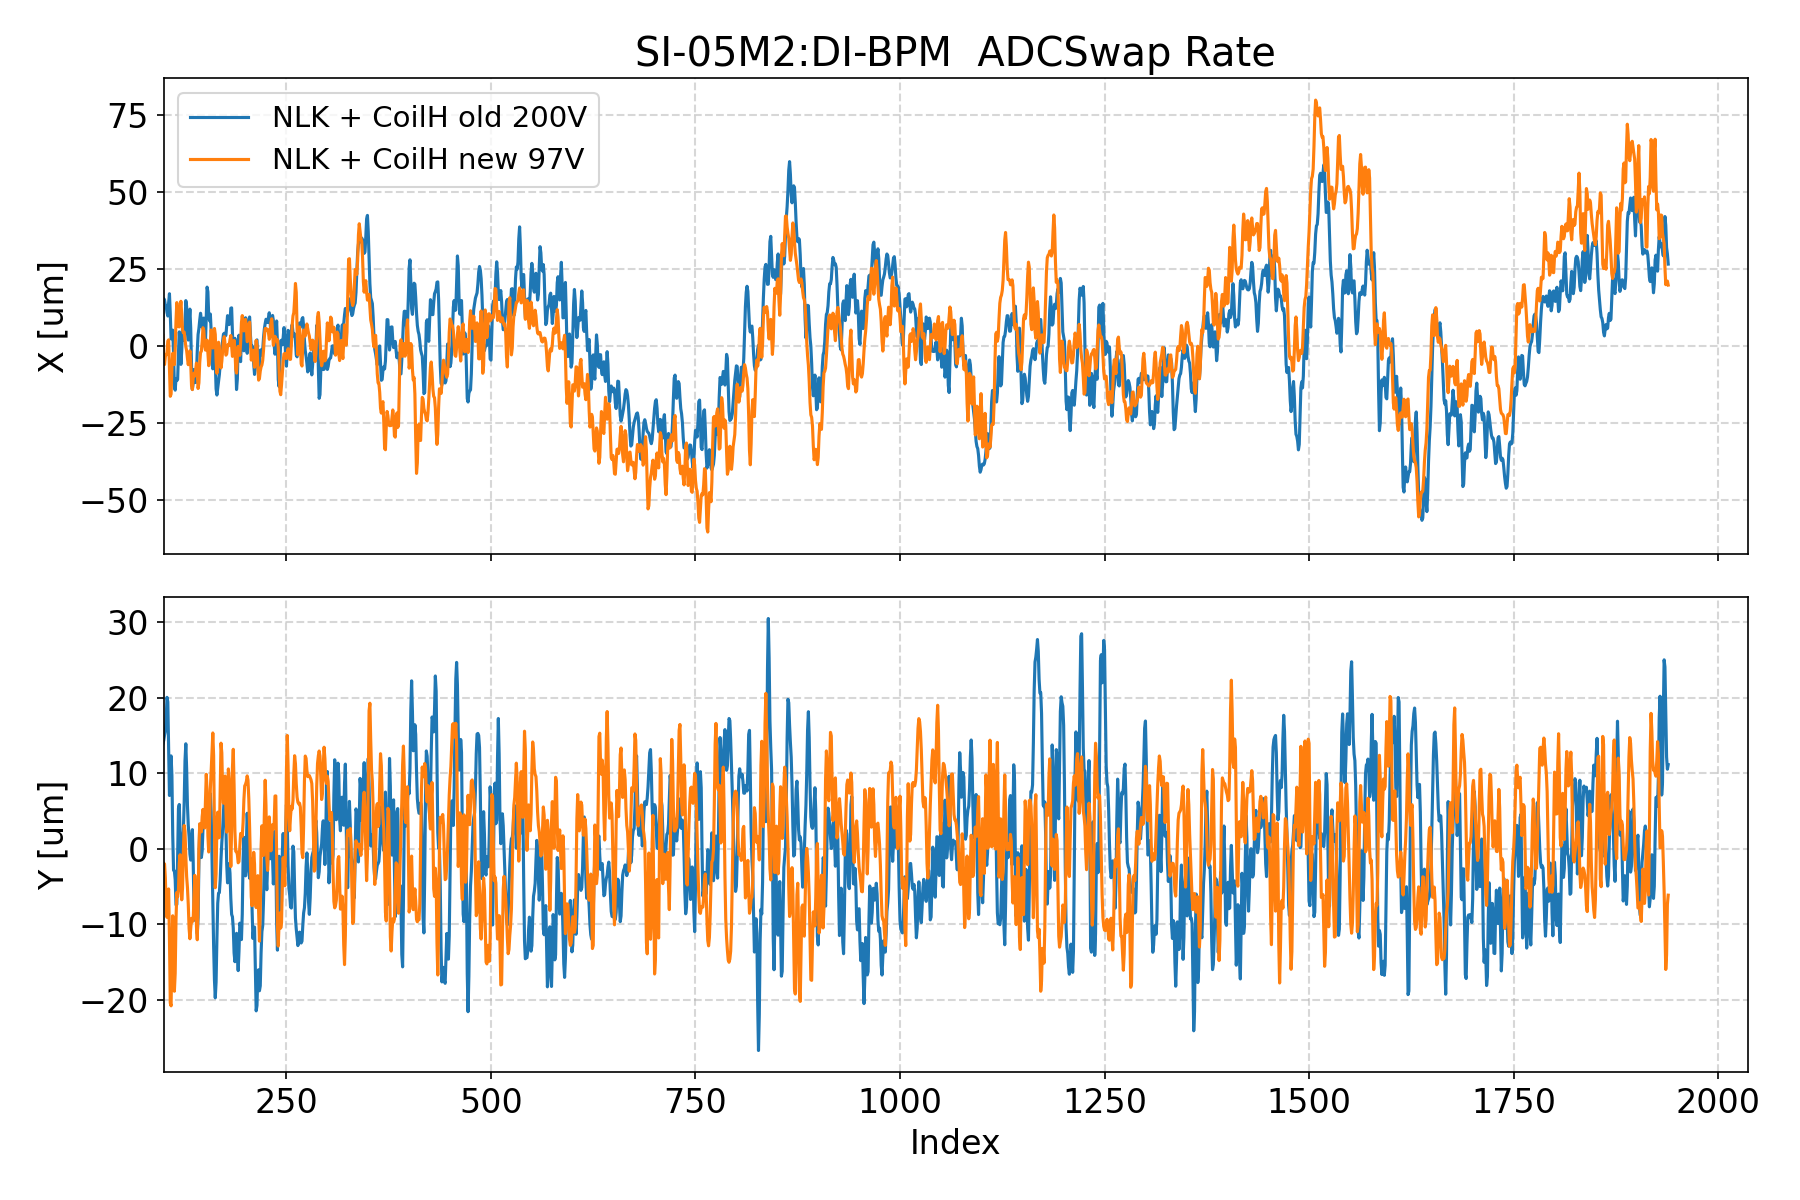
\includegraphics[width=0.8\textwidth]{2024-04-19/figures/nlk_and_coilh_old_new.png}
\end{frame}

\begin{frame}{Scan de amplitude (delay fixo)}
\centering
    Rms da taxa ADC Swap em 1 BPM (09M2) (taxa sub-TbT)
    \centering
    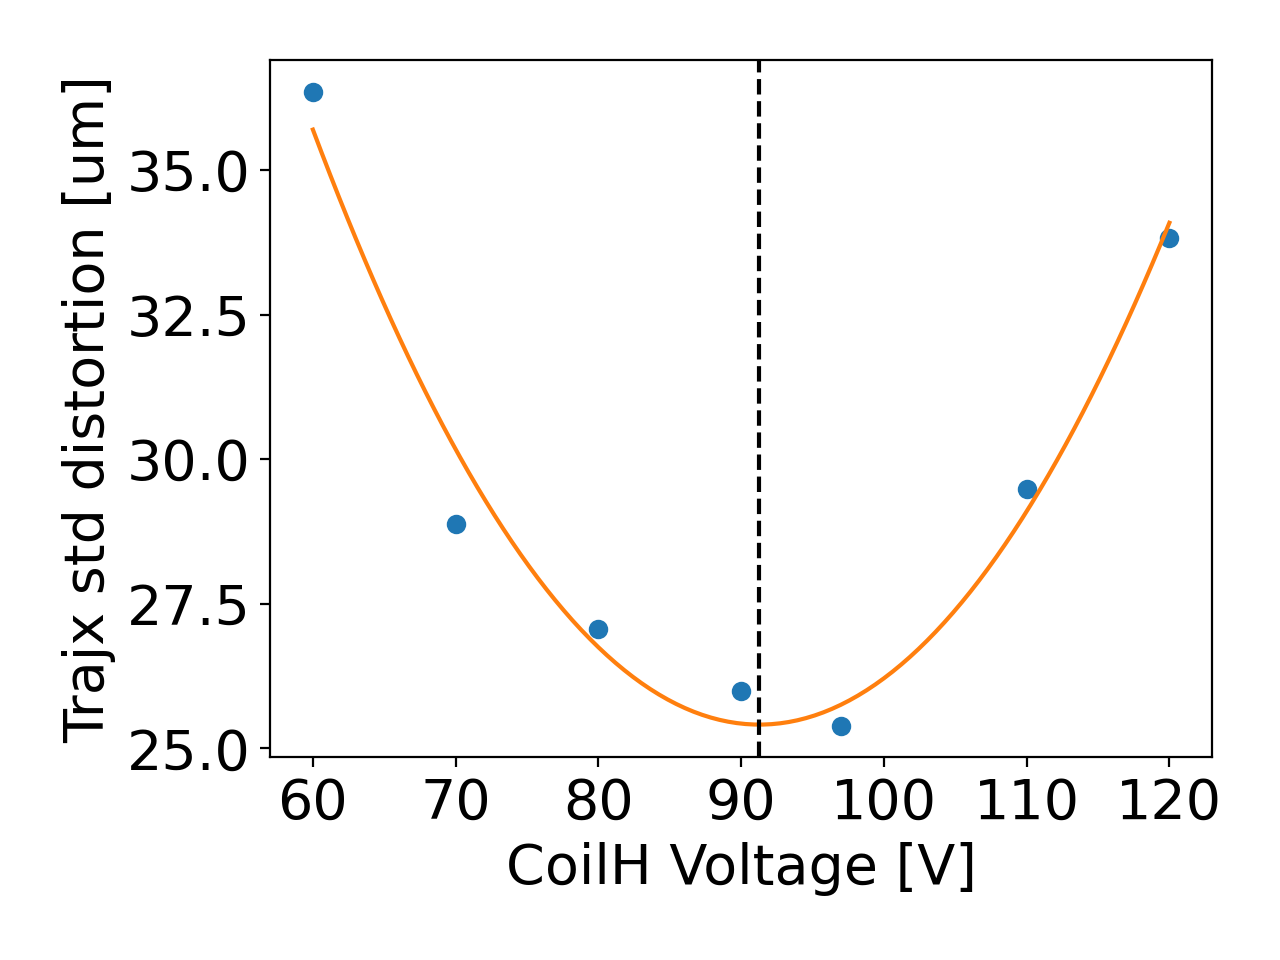
\includegraphics[width=0.8\textwidth]{2024-04-19/figures/voltage_scan_adcrate.png}

    Mínimo da distorção abaixo de 100V para esta temporização \\
    Ainda precisamos fazer scan de delay...
\end{frame}

\begin{frame}{Perturbação durante top-up}
    Trecho reto CARNAUBA (06SB), $x$ beam size 20$\mu$m
    \centering
    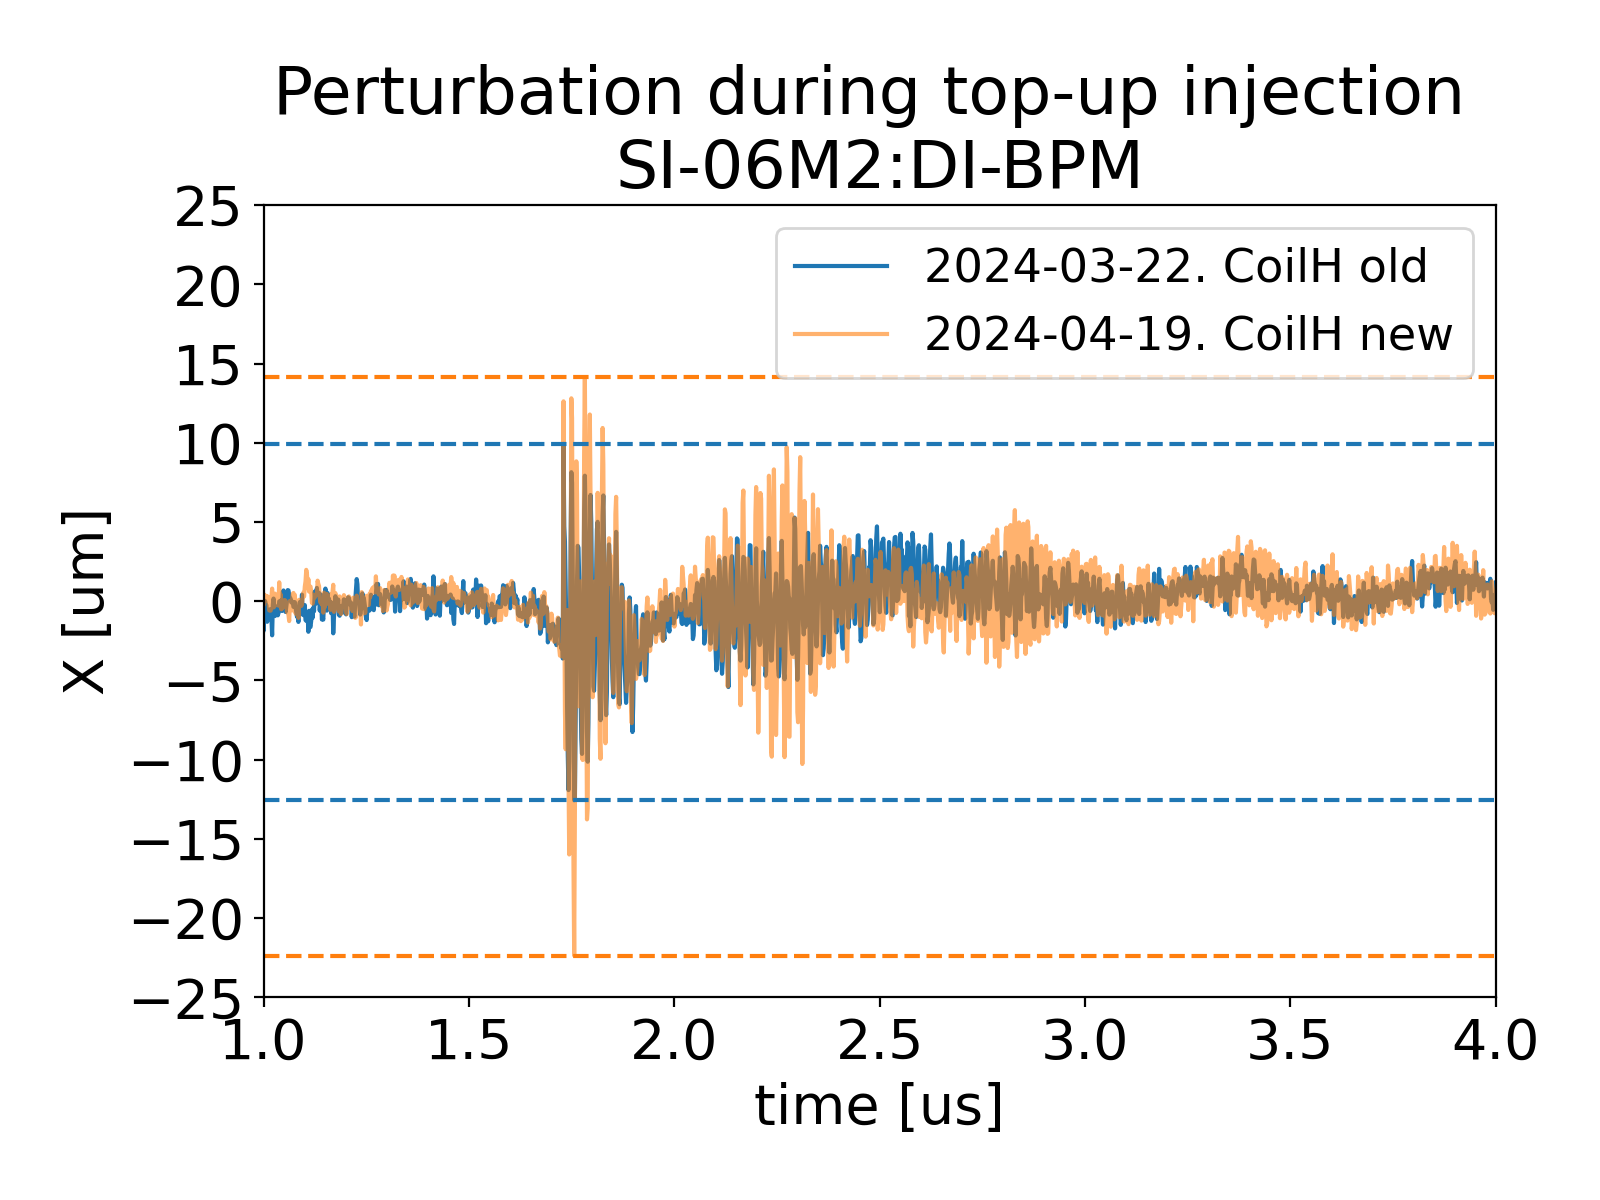
\includegraphics[width=0.8\textwidth]{2024-04-19/figures/injection_perturbSI-06M2:DI-BPM.png}
\end{frame}

\begin{frame}{Perturbação durante top-up}
    Trecho reto MANACÁ (09SA), $x$ beam size 65$\mu$m
    \centering
    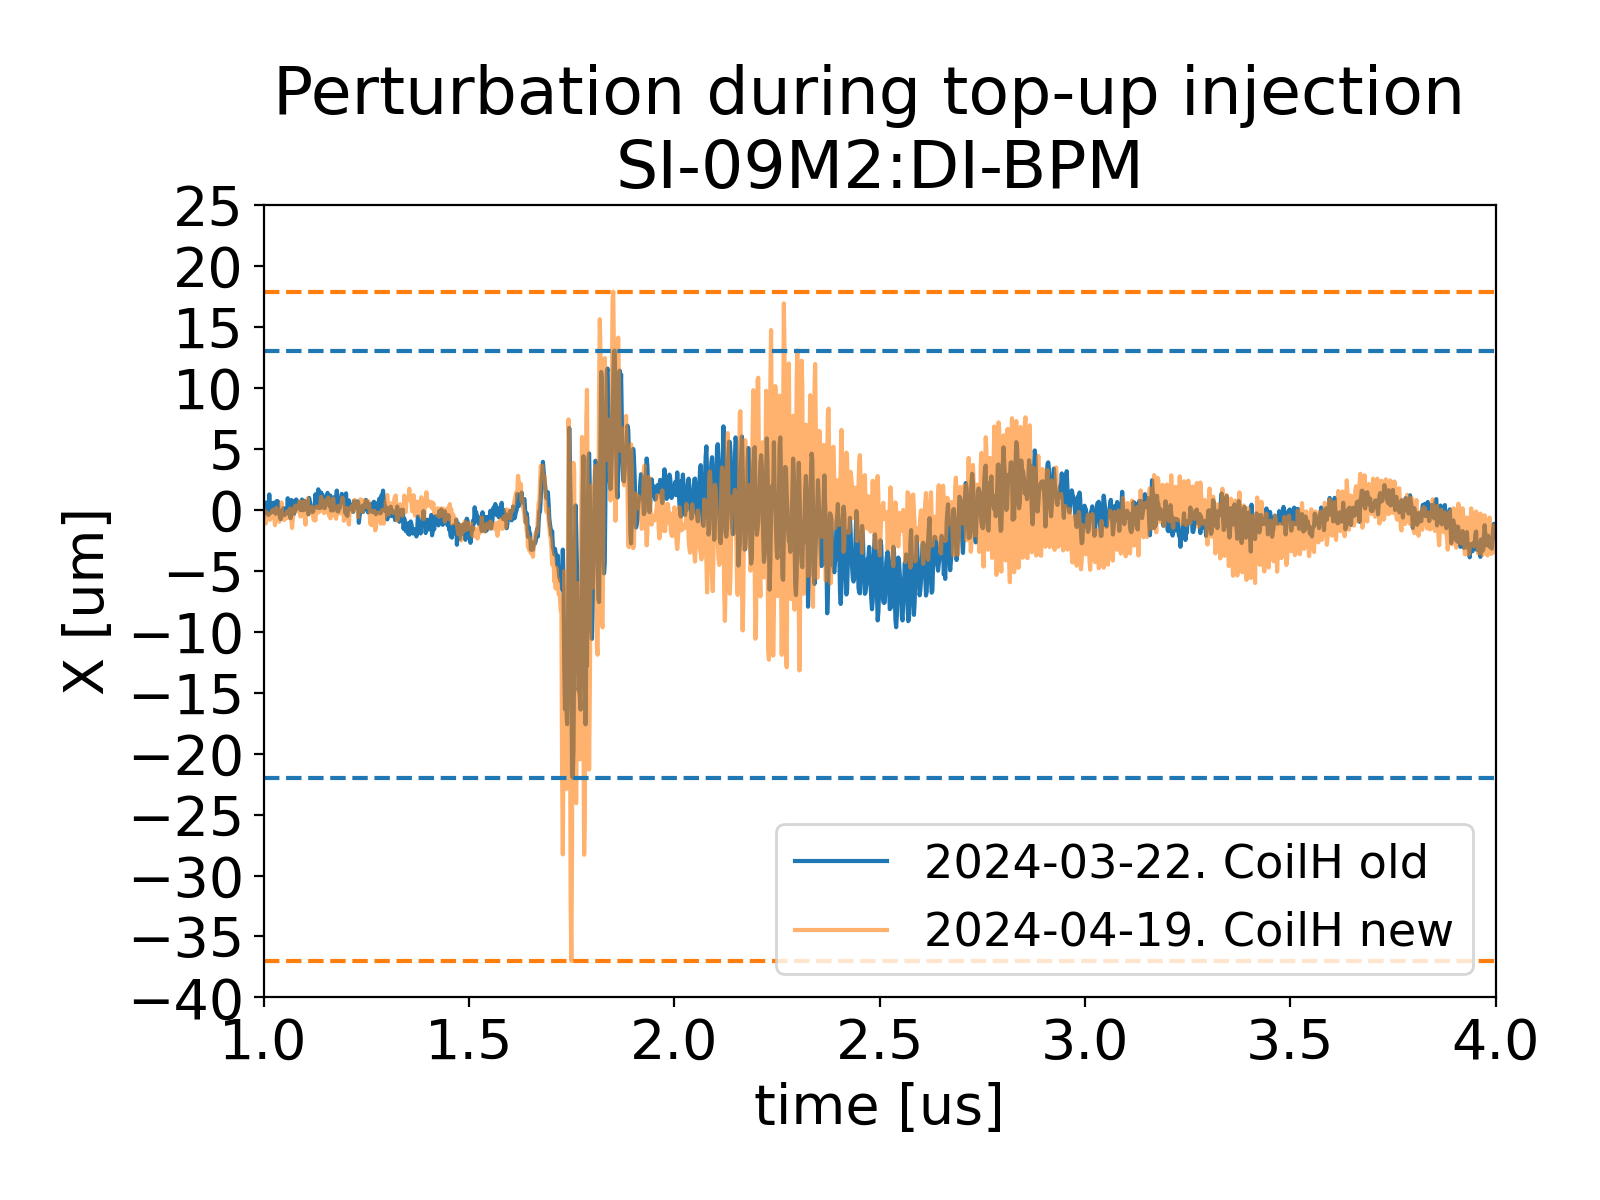
\includegraphics[width=0.8\textwidth]{2024-04-19/figures/injection_perturbSI-09M2:DI-BPM.png}

    Compensação está pior. Justifica voltar pro bastidor antigo logo? Podemos fazer mais estudos com feixe...
\end{frame}



%====================================================================
\section{Correção de bump na órbita do Booster}

\begin{frame}{Bump na órbita do booster}
\vspace{0.5cm}
\begin{itemize}
    \item Bump na órbita horizontal;
    \item Além do efeito de desvio de energia em função da variação de período de revolução, é invariante ao longo da rampa.
\vspace{0.5cm}
\end{itemize}
\centering
    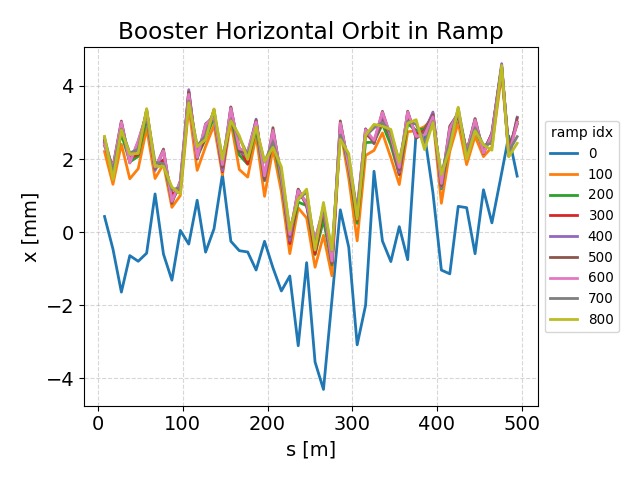
\includegraphics[scale=0.5]{2024-04-19/figures/bo-orbit.png}
\end{frame}

\begin{frame}{Correção com kicks nos QFs}
\vspace{0.5cm}
\begin{itemize}
    \item Estudo de adição de kicks nos QFs (deslocamentos)
    \item Correção em idx = 220 ($\approx 0.85 GeV$)
    \item "Best correctors": resíduo em função do número de QFs considerados na correção.
\vspace{0.5cm}
\end{itemize}
\centering
    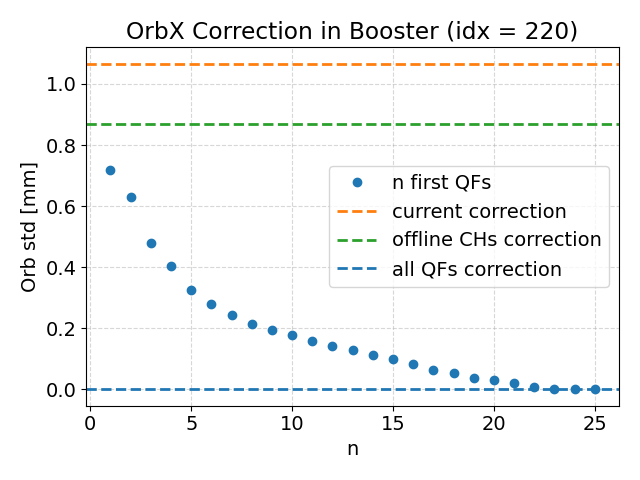
\includegraphics[scale=0.5]{2024-04-19/figures/qfs-correction.png}
\end{frame}

\begin{frame}{Correção com kicks com 10 QFs}
\vspace{0.5cm}
\begin{itemize}
    \item Resíduo maior em baixa energia
\vspace{0.5cm}
\end{itemize}
\centering
    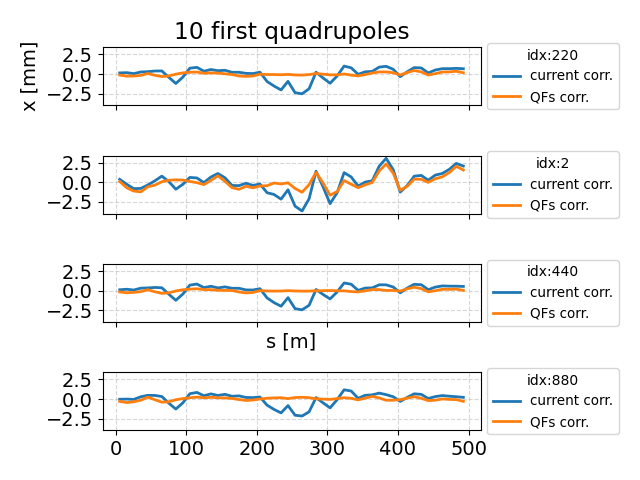
\includegraphics[scale=0.5]{2024-04-19/figures/bo-cod-corr-ramp.png}
\end{frame}

\begin{frame}{Deslocamentos dos QFs}
\vspace{0.5cm}
\centering
    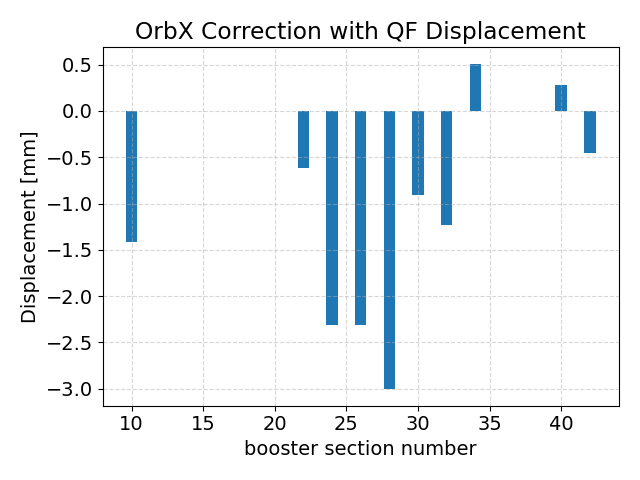
\includegraphics[scale=0.5]{2024-04-19/figures/qfs-displacements.png}
\end{frame}

%====================================================================
\end{document}